\documentclass[
  bibliography=totoc,     % Literatur im Inhaltsverzeichnis
  captions=tableheading,  % Tabellenüberschriften
  titlepage=firstiscover, % Titelseite ist Deckblatt
]{scrartcl}

% Paket float verbessern
\usepackage{scrhack}

% Warnung, falls nochmal kompiliert werden muss
\usepackage[aux]{rerunfilecheck}

% unverzichtbare Mathe-Befehle
\usepackage{amsmath}
% viele Mathe-Symbole
\usepackage{amssymb}
% Erweiterungen für amsmath
\usepackage{mathtools}

% Fonteinstellungen
\usepackage{fontspec}
% Latin Modern Fonts werden automatisch geladen
% Alternativ zum Beispiel:
%\setromanfont{Libertinus Serif}
%\setsansfont{Libertinus Sans}
%\setmonofont{Libertinus Mono}

% Wenn man andere Schriftarten gesetzt hat,
% sollte man das Seiten-Layout neu berechnen lassen
\recalctypearea{}

% Einrücken nach Absatz
\setlength{\parindent}{0pt}

% deutsche Spracheinstellungen
\usepackage{polyglossia}
\setmainlanguage{german}


\usepackage[
  math-style=ISO,    % ┐
  bold-style=ISO,    % │
  sans-style=italic, % │ ISO-Standard folgen
  nabla=upright,     % │
  partial=upright,   % ┘
  warnings-off={           % ┐
    mathtools-colon,       % │ unnötige Warnungen ausschalten
    mathtools-overbracket, % │
  },                       % ┘
]{unicode-math}

% traditionelle Fonts für Mathematik
\setmathfont{Latin Modern Math}
% Alternativ zum Beispiel:
%\setmathfont{Libertinus Math}

\setmathfont{XITS Math}[range={scr, bfscr}]
\setmathfont{XITS Math}[range={cal, bfcal}, StylisticSet=1]

% Zahlen und Einheiten
\usepackage[
  locale=DE,                   % deutsche Einstellungen
  separate-uncertainty=true,   % immer Fehler mit \pm
  per-mode=symbol-or-fraction, % / in inline math, fraction in display math
]{siunitx}

% chemische Formeln
\usepackage[
  version=4,
  math-greek=default, % ┐ mit unicode-math zusammenarbeiten
  text-greek=default, % ┘
]{mhchem}

% richtige Anführungszeichen
\usepackage[autostyle]{csquotes}

% schöne Brüche im Text
\usepackage{xfrac}

% Standardplatzierung für Floats einstellen
\usepackage{float}
\floatplacement{figure}{htbp}
\floatplacement{table}{htbp}
\setcounter{totalnumber}{5}

% Floats innerhalb einer Section halten
\usepackage[
  section, % Floats innerhalb der Section halten
  below,   % unterhalb der Section aber auf der selben Seite ist ok
]{placeins}

% Seite drehen für breite Tabellen: landscape Umgebung
\usepackage{pdflscape}

% Captions schöner machen.
\usepackage[
  labelfont=bf,        % Tabelle x: Abbildung y: ist jetzt fett
  font=small,          % Schrift etwas kleiner als Dokument
  width=0.9\textwidth, % maximale Breite einer Caption schmaler
]{caption}
% subfigure, subtable, subref
\usepackage{subcaption}

% Grafiken können eingebunden werden
\usepackage{graphicx}
% größere Variation von Dateinamen möglich
\usepackage{grffile}

% schöne Tabellen
\usepackage{booktabs}

% Verbesserungen am Schriftbild
\usepackage{microtype}

% Literaturverzeichnis
\usepackage[
  backend=biber,
  style=numeric,
  sorting=none
]{biblatex}


% Hyperlinks im Dokument
\usepackage[
  unicode,        % Unicode in PDF-Attributen erlauben
  pdfusetitle,    % Titel, Autoren und Datum als PDF-Attribute
  pdfcreator={},  % ┐ PDF-Attribute säubern
  pdfproducer={}, % ┘
]{hyperref}
% erweiterte Bookmarks im PDF
\usepackage{bookmark}

% Trennung von Wörtern mit Strichen
\usepackage[shortcuts]{extdash}

\author{%
  Frederik Rennebaum\\%
  \href{mailto:frederik.rennebaum@tu-dortmund.de}{frederik.rennebaum@udo.edu}%
  \texorpdfstring{\and}{,}%
  Martin Schönfeld\\%
  \href{mailto:martin.schoenfeld@tu-dortmund.de}{martin.schoenfeld@udo.edu}%
}
\publishers{TU Dortmund – Fakultät Physik}


\subject{VERSUCH NUMMER}
\title{TITEL}
\date{%
  Durchführung: DATUM
  \hspace{3em}
  Abgabe: DATUM
}

\begin{document}

\maketitle
\thispagestyle{empty}
\tableofcontents
\newpage
\setlength{\parindent}{0em} % keine Einrückungen nach Absatz

\section{Theorie}
\label{sec:Theorie}



In der Kernmagnetischen Resonanz (NMR) Spektroskopie werden die 
Relaxationszeiten T1 und T2 gemessen, um die Anordnung von Kernen 
in einem Molekül und ihre Wechselwirkungen mit der Umgebung zu untersuchen.

Die Relaxationszeit T1 ist die Zeit, die ein Kern benötigt, um von
seinem angeregten Zustand in seinen Grundzustand zurückzukehren. 
Sie wird gemessen, indem man den Kern durch ein kurzes Magnetfeldpulses
 anregt und dann die Zeit misst, die der Kern benötigt, um wieder in 
 seinen Grundzustand zurückzukehren.

Die Relaxationszeit T2 ist die Zeit, die ein Kern benötigt, um die 
Korrelation zwischen seinem Spin und dem Spin seiner Nachbarn zu 
verlieren. Sie wird gemessen, indem man





In der Kernmagnetischen Resonanz (NMR) Spektroskopie werden die 
Relaxationszeiten T1 und T2 mithilfe von Magnetfeldpulsen gemessen, 
um die Anordnung von Kernen in einem Molekül und ihre 
Wechselwirkungen mit der Umgebung zu untersuchen.

Die Relaxationszeit T1 ist die Zeit, die ein Kern benötigt, um 
von seinem angeregten Zustand in seinen Grundzustand zurückzukehren. 
Sie wird gemessen, indem man den Kern durch einen kurzen Magnetfeldpuls 
anregt und dann die Zeit misst, die der Kern benötigt, um wieder 
in seinen Grundzustand zurückzukehren. Dies wird durch die 
folgende Gleichung beschrieben:

\begin{equation}
    M(t) = M_0 e^{-t/T_1}
\end{equation}

wobei $M(t)$ die magnetische Ausrichtung des Kerns zum 
Zeitpunkt $t$ ist, $M_0$ die magnetische Ausrichtung des Kerns zum Zeitpunkt 0 ist, und $T_1$ die Relaxationszeit T1 ist.

Die Relax



In der gepulsten Kernmagnetischen Resonanz (NMR) 
Spektroskopie werden die Relaxationszeiten T1 und T2 mithilfe
 von Magnetfeldpulsen gemessen, um die Anordnung von Kernen in einem Molekül und ihre Wechselwirkungen mit der Umgebung zu untersuchen.

Die Relaxationszeit T1 ist die Zeit, die ein Kern benötigt, 
um von seinem angeregten Zustand in seinen Grundzustand 
zurückzukehren. Sie kann mithilfe verschiedener Verfahren 
gemessen werden, wie zum Beispiel dem 
Inversion-Recovery-Verfahren oder dem Carr-Purcell-Meiboom-Gill-Verfahren.

Das Inversion-Recovery-Verfahren basiert auf der Tatsache, 
dass die magnetische Ausrichtung von Kernen im angeregten 
Zustand um 180° invertiert wird, wenn sie von einem starken
 Magnetfeldpuls angeregt werden. Nach der Inversion wird 
 die magnetische Ausricht



Nachdem die magnetische Ausrichtung des Kerns durch den
 Inversionpuls um 180° invertiert wurde, kehrt der Kern 
 langsam in seinen Grundzustand zurück und die magnetische 
 Ausrichtung nimmt wieder zu. Die Relaxationszeit T1 
 kann aus der Zeit berechnet werden, die der Kern 
 benötigt, um wieder in seinen Grundzustand 
 zurückzukehren. Dies wird durch die folgende 
 Gleichung beschrieben:

\begin{equation}
M(t) = M_0 \left( 1 - 2e^{-t/T_1} \right)
\end{equation}

wobei $M(t)$ die magnetische Ausrichtung des Kerns zum 
Zeitpunkt $t$ ist, $M_0$ die magnetische Ausrichtung 
des Kerns zum Zeitpunkt 0 ist, und $T_1$ die 
Relaxationszeit T1 ist.

Das Carr-Purcell-Meiboom-Gill-Verfahren basiert auf 
der Anwendung von mehreren kurzen Magnetfeldpulsen, 
die den Kern anregen und seine magnetische 
Ausrichtung zerstören.



Die magnetische Ausrichtung des Kerns wird durch die 
Anwendung von mehreren kurzen Magnetfeldpulsen 
zerstört und kehrt danach langsam wieder in seinen 
Grundzustand zurück. Die Relaxationszeit T1 kann aus 
der Zeit berechnet werden, die der Kern benötigt, 
um wieder in seinen Grundzustand zurückzukehren. 
Dies wird durch die folgende Gleichung beschrieben:

\begin{equation}
M(t) = M_0 e^{-t/T_1}
\end{equation}

wobei $M(t)$ die magnetische Ausrichtung des Kerns
zum Zeitpunkt $t$ ist, $M_0$ die magnetische 
Ausrichtung des Kerns zum Zeitpunkt 0 ist, und $T_1$ 
die Relaxationszeit T1 ist.

Die Relaxationszeit T2 ist die Zeit, die ein Kern 
benötigt, um die Korrelation zwischen seinem Spin 
und dem Spin seiner Nachbarn zu verlieren. Sie kann 
mithilfe verschiedener Verfahren gemessen werden, 
wie zum Beispiel dem Spin-Echo-Verfahren oder dem Hahn-Echo-Verfahren.

Das Spin-Echo-Verfahren basiert auf der Anwendung 
von zwei Magnetfeldpulsen, die den Kern anregen 
und dann seine magnetische Ausrich



Das Spin-Echo-Verfahren basiert auf der Anwendung 
von zwei Magnetfeldpulsen, die den Kern anregen 
und dann seine magnetische Ausrichtung um 180° 
invertieren. Durch die Inversion wird die Korrelation
 zwischen dem Spin des Kerns und dem Spin 
 seiner Nachbarn wiederhergestellt und der Kern 
 kehrt in seinen Grundzustand zurück. Die 
 Relaxationszeit T2 kann aus der Zeit berechnet 
 werden, die der Kern benötigt, um wieder in 
 seinen Grundzustand zurückzukehren. Dies wird 
 durch die folgende Gleichung beschrieben:

\begin{equation}
M(t) = M_0 e^{-t/T_2}
\end{equation}

wobei $M(t)$ die magnetische Ausrichtung des 
Kerns zum Zeitpunkt $t$ ist, $M_0$ die magnetische
 Ausrichtung des Kerns zum Zeitpunkt 0 ist, und 
 $T_2$ die Relaxationszeit T2 ist.

Das Hahn-Echo-Verfahren basiert auf der 
Anwendung von drei Magnetfeldpulsen, die den 
Kern anregen und dann seine magnetische 
Ausrichtung um 180° invertieren. Durch die 
Inversion wird die Korrelation zwischen dem 
Spin des Kerns und dem Spin seiner Nachbarn 
wiederhergestellt und der Kern kehrt in 
seinen Grundzustand zurück. Die Relaxationszeit 
T2 kann aus der Zeit berechnet werden, 
die der Kern benötigt, um wieder in seinen 
Grundzustand zurückzukehren. Dies wird 
durch die folgende Gleichung beschrieben:

\begin{equation}
M(t) = M_0 \cos \left( \frac{\pi t}{T_2} \right)
\end{equation}

wobei $M(t)$ die magnetische Ausrichtung 
des Kerns zum Zeitpunkt $t$ ist, $M_0$



wobei $M(t)$ die magnetische Ausrichtung 
des Kerns zum Zeitpunkt $t$ ist, $M_0$ 
die magnetische Ausrichtung des Kerns zum
 Zeitpunkt 0 ist, und $T_2$ die Relaxationszeit T2 ist.

Durch die Messung von T1 und T2 können 
wichtige Informationen über die Anordnung
 von Kernen in einem Molekül und ihre 
 Wechselwirkungen mit der Umgebung gewonnen 
 werden. Die Relaxationszeiten hängen 
 von verschiedenen Faktoren ab, wie zum 
 Beispiel der Lage des Kerns im Molekül, 
 seiner chemischen Umgebung und der Temperatur.

In unserem Praktikum haben wir gepulste
 NMR-Spektroskopie betrieben und die 
 Relaxationszeiten T1 und T2 mithilfe des 
 Inversion-Recovery-Verfahrens und 
 des Carr-Purcell-Meiboom-Gill-Verfahrens 
 gemessen. Die erhaltenen Ergebnisse 
 werden im folgenden Abschnitt diskutiert.



\section{Durchführung}
\label{sec:Durchführung}

\subsection{Justage}

    Zunächst werden gemäß der Anleitung Startparameter eingestellt.
    Dann wird die Frequenz feinabgestimmt

    feinabstimmung damit keine schwingung mehr auftritt
    phase einstllen damit alles auf realteil liegt
    feldhomogenität maximieren, indem FID versucht wird zu maximieren 
    indem der Gradient eingestellt wird

    Pulslänge einstellen "A" und B"

    \begin{figure}[htbp]
        \centering
        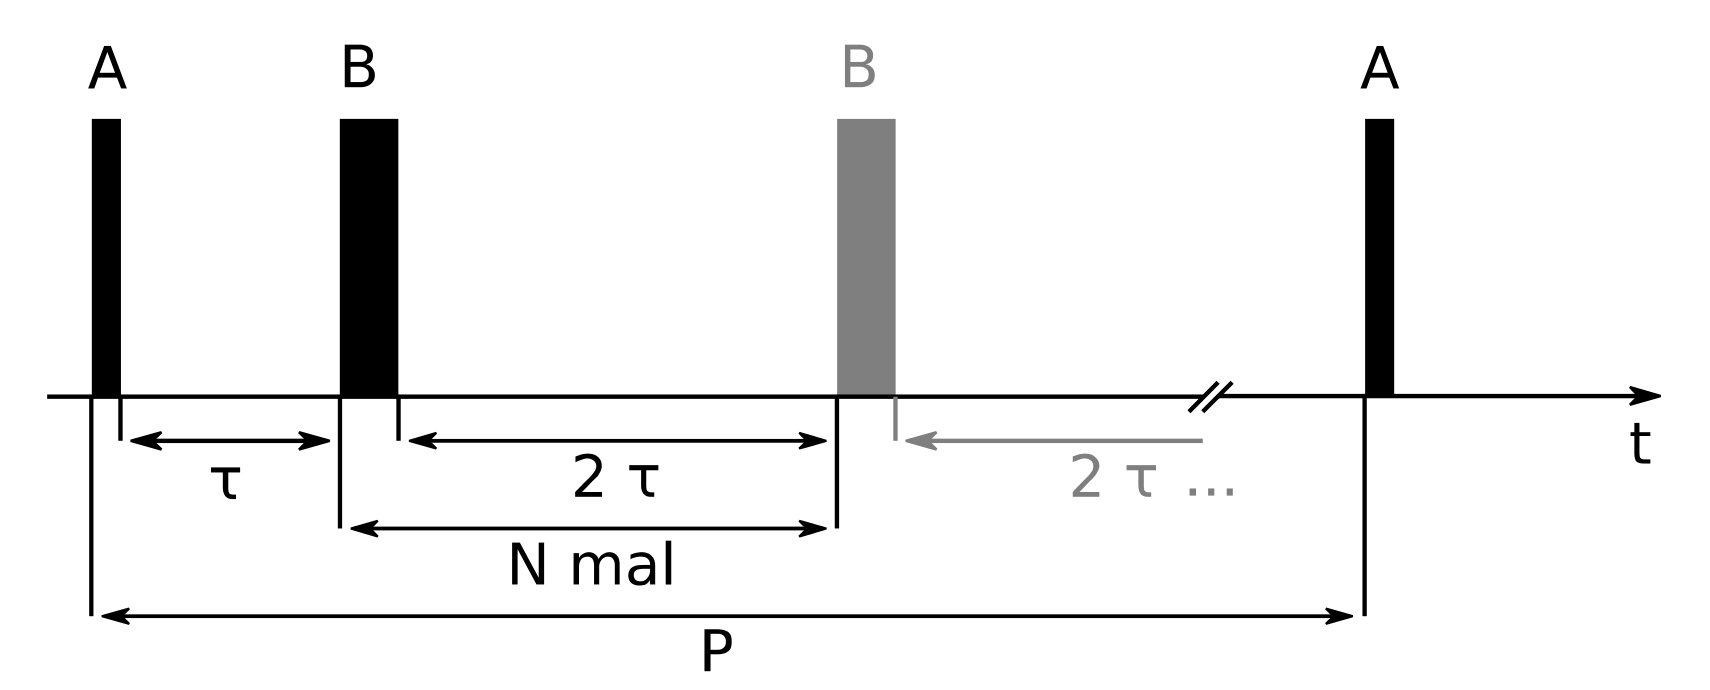
\includegraphics[width=\textwidth]{figures/pulsprogramm.png}
        \caption{<caption>}
        \label{<label>}
    \end{figure}

    

\subsection{}
\subsection{Justage}
\subsection{Justage}


\section{Auswertung}
\label{sec:Auswertung}

\section{Diskussion}
\label{sec:Diskussion}

% fehlerquellen:#

Bei der Betrachtung der Justage Messung fällt auf dass eine geringere Schrittweite
von Vorteil gewesen wäre für genauere Bestimmung der Strahlbreite z.B.
Auch die Bestimmung des Geometriewinkels aus dem Rocking Scan war aufgrund dieses Grundes
nicht sehr genau möglich. 
Der Geometriewinkel weicht um ca. $40 \%$ dem Theorie Wert (über den Z-scan) ab.

Der manuelle Fit war schwierig passend einzustellen so dass immer eine Seite
nicht richtig gepasst hat.
Demnach passt der Fit aber im Bereich von ca. $\SI{0.5}{\degree}$ bis $\SI{0.9}{\degree}$
optisch gut.
Aufgrund der manuellen Anpassung von 7 Parameter ist zu erwarten
keine sehr gute Anpassung hinzubekommen.
Ein weiterer Grund für Abweichungen von der Theorie Kurve sind Abnutzungen der Probe.

Für den kritischen Winkel lässt sich eine 
dementsprechend große Abweichungen von über 
$88 \%$ beobachten.  
$\alpha_\text{c,PS,gemessen} = \SI{0.081}{\degree}$ zu dem Literaturwert 
$\alpha_\text{c,PS,Literatur} = \SI{0.153}{\degree}$\cite{anleitung} 

Die Schichtdicke des Polysterol-Films, welche über den Parratt-Algorithmus bestimmt wurde,
 weicht jedoch nur um $5,19 \%$ zu der Schichdickenbestimmung über die Mittelung der Oszillationsminima ab.
Die Korrektur des Brechungsindizes von Silizium trifft annähernd den Literaturwert, $\delta_\text{PS,Literatur} = \num{7.6e-6}$\cite{anleitung},
 und weicht um $\approx 2,7 \%$ ab.

% d_\text{PS} = \SI{8.52+-0.26e-08}{\meter}
% z_2 &= \SI{8.10e-8}{\meter}\\

% \begin{align*}
%     \alpha_\text{c,PS} &= \SI{0.081}{\degree} \\
%     \alpha_\text{c,Si} &= \SI{0.220}{\degree}
% \end{align*}
% berechnet werden



\printbibliography{}

\end{document}



% nützliche Layouts Idee: als shortcut in script_helper

% \begin{figure}
%   \centering
%   \includegraphics[width=0.7\textwidth]{content/BILD.png}
%   \caption{BESCHREIBUNG \cite{Anleitung}.}
%   \label{fig:LABEL}
% \end{figure}




% \begin{table}
%   \centering
%   \caption{BESCHREIBUNG.}
%   \label{tab:LABEL}
%   \begin{tabular}{S S}
%     \toprule
%       \multicolumn{1}{c}{} &
%       \multicolumn{1}{c}{$U_B = 180V $} &
%
%     \midrule
%     {$ D \;/\; \si{\milli\meter}$} &
%     {$ U_d \;/\; \si{\volt}$} \\
%
%     \midrule
%        6	& 19.8 &	21.7 &	 25	  & 29.3 & 	32.7 \\
%       12	& 16.5 &	18.6 &	 21.4 &	25.4 & 	27.4 \\
%
%     \bottomrule
%   \end{tabular}
% \end{table}




% \begin{equation}
%
%     \label{eqn:LABEL}
% \end{equation}
